\documentclass[letterpaper, 11pt]{article}
\usepackage[margin=1in]{geometry}

% Set the typeface to Times Roman
\usepackage{times}

%\usepackage{hyperref}
\usepackage{amsfonts}%
\usepackage{amssymb}%
\usepackage{amsthm}% allows theoremstyles (see below) and provides a proof environment
\usepackage{bm}
\usepackage{relsize}
\usepackage{graphicx}
\usepackage{caption}
\usepackage{epstopdf}
\usepackage{amsmath}
\usepackage{tikz}
\usetikzlibrary{trees,arrows}
\usetikzlibrary{decorations}
\usetikzlibrary[decorations]
\usepgflibrary{decorations.pathmorphing}
\usepgflibrary[decorations.pathmorphing]
\usetikzlibrary{decorations.pathmorphing}
\usetikzlibrary[decorations.pathmorphing]
\usepackage{booktabs}
\usepackage[authoryear]{natbib}
\usepackage{subcaption}
\usepackage{pseudocode}
\usepackage{centernot}
%\usepackage{float}
\usepackage{verbatim} %% for commenting blocks
\usepackage[authoryear]{natbib}
\usepackage{url}

\bibpunct{(}{)}{,}{}{}{;} %% added this to make \citep{x} use parentheses

\newcommand{\problemAnswer}[1]{%#1% Defines the problem answer command with the content as the only argument
\noindent\framebox[0.95\columnwidth][c]{\begin{minipage}{0.92\columnwidth}\color{blue}{#1}\end{minipage}} % Makes the box around the problem answer and puts the content inside
}

%% independence symbol and expectation operator %%
\newcommand\independent{\protect\mathpalette{\protect\independenT}{\perp}}
\def\independenT#1#2{\mathrel{\rlap{$#1#2$}\mkern2mu{#1#2}}}

\DeclareMathOperator{\circlearrow}{\hbox{$\circ$}\kern-1.5pt\hbox{$\rightarrow$}}
\DeclareMathOperator{\circlecircle}{\hbox{$\circ$}\kern-1.2pt\hbox{$--$}\kern-1.5pt\hbox{$\circ$}}

\DeclareMathOperator{\an}{an}
\DeclareMathOperator{\pa}{pa}
\DeclareMathOperator{\ch}{ch}
\DeclareMathOperator{\pre}{pre}
\DeclareMathOperator{\de}{de}
\DeclareMathOperator{\nd}{nd}
\DeclareMathOperator{\sib}{sib}
\DeclareMathOperator{\dis}{dis}
\DeclareMathOperator{\mb}{mb}
\DeclareMathOperator{\doo}{do}
\DeclareMathOperator{\odds}{\text{OR}}
\DeclareMathOperator*{\argmax}{arg\,max}
\DeclareMathOperator*{\argmin}{arg\,min}
\definecolor{lemon}{RGB}{ 242, 200,  24}
\def\ci{\perp\!\!\!\perp}
\newcommand{\E}{\mathbb{E}}
\newcommand{\G}{\mathcal{G}}

\newcommand\indep{\protect\mathpalette{\protect\independenT}{\perp}}
\def\independenT#1#2{\mathrel{\rlap{$#1#2$}\mkern2mu{#1#2}}}

\newtheorem{Lma}{Lemma}
\newtheorem{Thm}{Theorem}

\DeclareMathOperator{\diedgeright}{\textcolor{blue}{\boldsymbol{\rightarrow}}}
\DeclareMathOperator{\diedgeleft}{\textcolor{blue}{\boldsymbol{\leftarrow}}}
\DeclareMathOperator{\biedge}{\textcolor{red}{\boldsymbol{\leftrightarrow}}}
\DeclareMathOperator{\udedge}{\textcolor{brown}{\boldsymbol{\textendash}}}
%%%%%%%%%%%%%%%%%%%%%%%%%%%%

\title{CS 476/676 (Spring 2021): Homework 2}

\author{}

\date{Due: Feb 17, 2021 at 11:59pm EST}

\begin{document}

\maketitle

\setlength{\parindent}{0em}
\setlength{\parskip}{0.8em}

\large\textbf{Name:} \underline{\hspace{30pt} \color{blue} Josh Popp \hspace{30pt}}
\vspace{1em}

	\textbf{Instructions}: This homework requires answering some open-ended questions, short proofs, and
	programming. This is an individual assignment, not group work. Though you may
	discuss the problems with your classmates, you must solve the problems and
	write the solutions independently. As stated in the syllabus, copying code
	from a classmate or the internet (even with minor changes) constitutes
	plagiarism. You are required to submit your answers in pdf form (use \LaTeX)
	in a file called \texttt{<your-JHED>-hw2.pdf} to Gradescope under ``HW2''. Code should be submitted also to Gradescope under ``HW2 Programming''. Note that the autograder setup is intended only to register submission of the code, and will not provide any feedback. Code grading will be performed manually.
	Late submissions will be penalized, except in extenuating circumstances such
	as medical or family emergency. Submissions submitted 0-24 hours late will be
	penalized 10\%, 24-48 hours late by 20\%, 48-72 hours late by 30\%, and later
    than 72 hours by 100\%. Late days may be used (if available) to avoid these penalties.

    The total assignment is worth 85 points.

\vspace{1em}

{\large\textbf{Problem 1}} (5 points)

Briefly explain (for both senses of completeness) the statement -- ``d-separation is \emph{sound} and \emph{complete} for detecting conditional independences in statistical models of a DAG where all variables are observed.'' 2-3 paragraphs of explanation are sufficient.

\problemAnswer{
Given our DAG $\G$ with all variables $\{ V_i \}$ observed, we can choose any probability distribution $p(V)$ that's compatible with $\G$, and under that probability distribution any two nodes $A$ and $B$ that are d-separated by a set of conditioning observations $C$ are conditionally independent given those conditioning observations, so $p(A,B \mid C)=p(A \mid C)p(B \mid C)$. This property of d-separation is referred to as soundness. On the flip side, d-separation is also weakly complete, meaning that if $A$ and $B$ {\bf aren't} d-separated in $\G$, then there exists a distribution $p$ such that $p(A,B \mid C) \neq p(A \mid C)p(B \mid C)$. This is considered weak completeness because it's possible that $p(A,B \mid C) = p(A \mid C)p(B \mid C)$ via exact cancellation, where independence is non-graphical but technically the aforementioned factorization does hold. \\ \\
We can move beyond this possibility of non-graphical independence through the faithfulness assumption, restricting our scope of factorizations/ distributions $p$ to distributions where non-graphical conditional independences are not possible. With this restriction, the soundness property of d-separation holds, so any d-separated nodes are conditionally independent, and now the reverse holds true that any non-d-separated nodes are also not conditionally independent.
}

\vspace{1em}

{\large\textbf{Problem 2}} (15 points)

\begin{figure}[h]
	\begin{center}
		\scalebox{0.7}{
			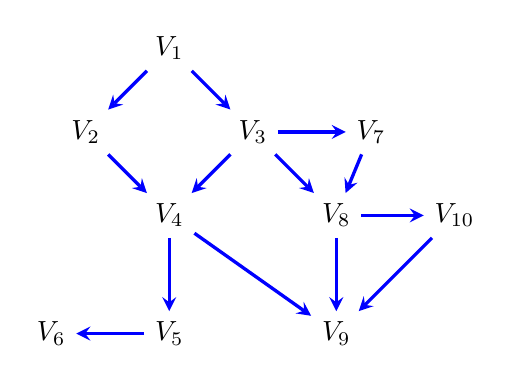
\begin{tikzpicture}[>=stealth, node distance=1.5cm]
			\tikzstyle{format} = [draw, thick, circle, minimum size=1.0mm, inner sep=0pt]
			\tikzstyle{square} = [draw, thick, minimum size=1.0mm, inner sep=3pt]
			\begin{scope}
			\path[->, very thick]
			node[] (x1) {$V_1$}
			node[below left of=x1] (x2) {$V_2$}
			node[below right of=x1] (x3) {$V_3$}
			node[right of=x3] (x7) {$V_7$}
			node[below right of=x3] (x8) {$V_8$}
			node[below left of=x3] (x4) {$V_4$}
			node[right of=x8] (x10) {$V_{10}$}
			node[below of=x8] (x9) {$V_9$}
			node[below of=x4] (x5) {$V_5$}
			node[left of=x5] (x6) {$V_6$}
			(x1) edge[blue] (x2)
			(x1) edge[blue] (x3)
			(x2) edge[blue] (x4)
			(x3) edge[blue] (x7)
			(x3) edge[blue] (x4)
			(x3) edge[blue] (x8)
			(x4) edge[blue] (x5)
			(x4) edge[blue] (x9)
			(x5) edge[blue] (x6)
			(x7) edge[blue] (x8)
			(x8) edge[blue] (x9)
			(x8) edge[blue] (x10)
			(x10) edge[blue] (x9)
			;
			\end{scope}
			\end{tikzpicture}
		}
	\end{center}
	\caption{}
	\label{fig:prob1}
\end{figure}

Refer to Figure~\ref{fig:prob1} for this problem.

1) Assuming $V_1, \dots, V_{10}$ are binary random variables, how many parameters are required to specify the full joint distribution $p(V)$ without a graphical model? (3 points)

\problemAnswer{
$$p(V)=\prod_{i=1}^{10}p(V_i \mid \{ V \} \setminus \{ V_i \})$$
Each node has one parameter for each of the $2^9$ possible configurations of the other 9 nodes in the graph. This means we'll need $10*(2^9)$ parameters for the full joint distribution $p(V)$.
}

2) Assuming binary random variables, how many parameters are required to specify the joint distribution using the DAG factorization for Figure~\ref{fig:prob1}? Show your work. (5 points)

\problemAnswer{
Each node $V_i$ still needs one parameter for each ($2^{n_i}$) possible configuration of its $n_i$ parents, but now each node has a limited number of parents $n_i \leq 9$.
\begin{align*}
V_1,\ n_1=0,&\ \ \ \ \ \ 1 \textrm{ parameters}\\
V_2,\ n_2=1,&\ \ \ \ \ \ 2 \textrm{ parameters}\\
V_3,\ n_3=1,&\ \ \ \ \ \ 2 \textrm{ parameters}\\
V_4,\ n_4=2,&\ \ \ \ \ \ 4 \textrm{ parameters}\\
V_5,\ n_5=1,&\ \ \ \ \ \ 2 \textrm{ parameters}\\
V_6,\ n_6=1,&\ \ \ \ \ \ 2 \textrm{ parameters}\\
V_7,\ n_7=1,&\ \ \ \ \ \ 2 \textrm{ parameters}\\
V_8,\ n_8=2,&\ \ \ \ \ \ 4 \textrm{ parameters}\\
V_9,\ n_9=3,&\ \ \ \ \ \ 8 \textrm{ parameters}\\
V_{10},\ n_{10}=1,&\ +2 \textrm{ parameters}
\end{align*}
For a total of 29 parameters
}

3) Answer the following d-separation queries and for any queries where they are not d-separated, provide at least one active/unblocked path. Is

a) $V_2 \ci_{\ \text{d-sep}} V_9 \mid V_4$? \\
b) $V_7 \ci_{\ \text{d-sep}} V_5 \mid V_3, V_8$? \\
c) $V_2, V_4 \ci_{\ \text{d-sep}} V_7 \mid V_6, V_9, V_{10}$?

(7 points)

\problemAnswer{
a) No, $V_3 \diedgeright V_8 \diedgeright V_9$ is open, and conditioning on $V_4$ opens up a path from $V_2 \diedgeright V_3$ \\
b) Yes, they are d-separated \\
c) No, there is a tail-to-tail connection from $V_4$ to $V_7$, and since we conditioned on $V_6$, a common descendant of $V_2$ and $V_3$, there is also a path from $V_2$ to $V_7$ through $V_3$.
}

\vspace{2em}

{\large\textbf{Problem 3}} (30 points)

\begin{figure}[h]
	\begin{center}
		\scalebox{0.8}{
			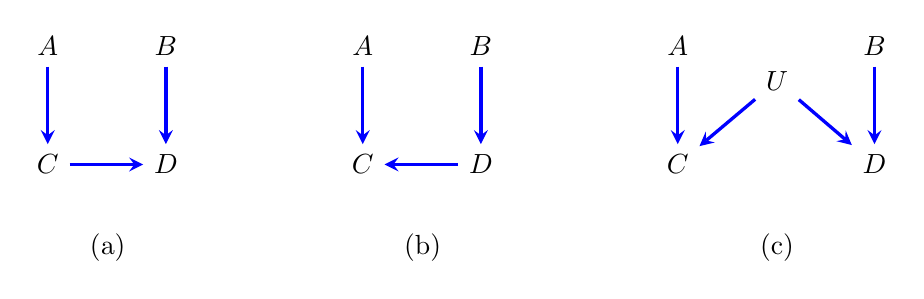
\begin{tikzpicture}[>=stealth, node distance=1.5cm]
			\tikzstyle{format} = [draw, thick, circle, minimum size=1.0mm, inner sep=0pt]
			\tikzstyle{square} = [draw, thick, minimum size=1.0mm, inner sep=3pt]
			\begin{scope}
			\path[->, very thick]
			node[] (a) {$A$}
			node[right of=a] (b) {$B$}
			node[below of=a] (c) {$C$}
			node[right of=c] (d) {$D$}
			node[below right of=c, xshift=-0.3cm] (label) {(a)}
			(a) edge[blue] (c)
			(b) edge[blue] (d)
			(c) edge[blue] (d)
			;
			\end{scope}

			\begin{scope}[xshift=4cm]
			\path[->, very thick]
			node[] (a) {$A$}
			node[right of=a] (b) {$B$}
			node[below of=a] (c) {$C$}
			node[right of=c] (d) {$D$}
			node[below right of=c, xshift=-0.3cm] (label) {(b)}
			(a) edge[blue] (c)
			(b) edge[blue] (d)
			(d) edge[blue] (c)
			;
			\end{scope}

			\begin{scope}[xshift=8cm]
			\path[->, very thick]
			node[] (a) {$A$}
			node[right of=a, xshift=1cm] (b) {$B$}
			node[below of=a] (c) {$C$}
			node[right of=c, xshift=1cm] (d) {$D$}
			node[above right of=c, xshift=0.2cm] (u) {$U$}
			node[below right of=c, xshift=0.2cm] (label) {(c)}
			(a) edge[blue] (c)
			(b) edge[blue] (d)
			(u) edge[blue] (c)
			(u) edge[blue] (d)
			;
			\end{scope}
			\end{tikzpicture}
		}
	\end{center}
	\caption{}
	\label{fig:prob2}
\end{figure}

Refer to Figure~\ref{fig:prob2} for this problem. Say we are given data on four variables $A, B, C, \text{ and } D$ (observed variables) and are unable to obtain data on the variable $U.$ Answer the following questions:

1) Describe qualitatively how the causal interpretations for (a), (b), and (c) are different from each other. A few sentences/a paragraph is sufficient. (3 points)

\problemAnswer{
In all cases, $A$ causes $C$, $B$ causes $D$, and there's some relationship betwen $C$ and $D$. In (a), $C$ causes $D$. In (b), $D$ causes $C$. In (c), $C$ and $D$ are both caused by an unobserved variable $U$.
}

2) List all independences that comprise the local Markov property for the DAGs in (a) and (b). Based on these two lists, identify independences present in (a) but not in (b), and vice versa. (5 points)

\problemAnswer{
(a) \begin{align*}
A &\ci B \\
B &\ci A \\
C &\ci B \mid A \\
D &\ci A \mid C,B
\end{align*}
(b) \begin{align*}
A &\ci B \\
B &\ci A \\
C &\ci B \mid D,A \\
D &\ci A \mid B
\end{align*}
The latter two independences in both lists are specific to that DAG due to the change in causal relationship between $C$ and $D$
}

3) Use d-separation to identify a \textbf{set} of conditional independences implied over the \textbf{observed} variables in (c) that is unique to (c), i.e., this set should not be implied in (a) and (b). (5 points)

\problemAnswer{
\{ $(A \ci B\mid C)$, $(A \ci B \mid D)$ \}
}

4) Based on your answers to 2) and 3), and assuming that the true data generating process for $A, B, C, D,$ and $U$ corresponds to an NPSEM-IE defined over one of the DAGs shown in Figure~\ref{fig:prob1}, describe  how you would construct a series of statistical hypothesis tests to arrive at the true causal DAG.\footnote{Ignore, for now, issues related to multiple testing (if you are aware of what that is.)} What is the underlying assumption used to ensure that these tests allow us to choose between these structures that imply different d-separation statements? (7 points)

\problemAnswer{
Let's consider two null hypotheses: $H_{0,1}=A \ci B \mid C$, and $H_{0,2}=A \ci B \mid D$ and use process of elimination to settle on a true causal DAG. Rejecting a null hypothesis amounts to rejecting the corresponding DAG. If we reject $H_{0,1}$ but fail to reject $H_{0,2}$, then we should assume (b) is the true causal DAG (since under (b) we see that $A {\centernot{\ci}} B \mid C$ but $A \ci B \mid D$). If we reject $H_{0,2}$ but fail to reject $H_{0,1}$, then we can adopt (a) as the causal DAG. If we fail to reject either null, we assume (c) is the true causal DAG - and if we reject both, then there's either something wrong with our statistical test or our models. For statistical testing, we can use bootstrapping to obtain a confidence interval for each odds ratio $\odds(A,B \mid C)$ and $\odds(A,B \mid D)$. Relying on the fact that $\odds(A,B \mid C)=1 \iff A \ci B \mid C$, we can then obtain a p-value from these confidence intervals, and if this p-value falls below a user-specified threshold $\alpha$ then we reject the corresponding null hypothesis. This relies on the assumption that this test statistic is valid for (and only for) DAGs in which $A$ and $B$ are d-separated given $C$, which is why we can only use process of elimination.
}

5) Now imagine that the edges $A \diedgeright D$ and $B \diedgeright C$ were also present in the DAGs shown in (a), (b), and (c). Show that these new DAGs are \textbf{not} statistically distinguishable using observed data. (5 points)

\problemAnswer{
Write your answer here.
\vspace*{50pt}
}

6) Summarize, in a few sentences, what the above exercise tells you about the use of statistical tests in the statistical model of a DAG to learn information regarding causal models of a DAG. (5 points)

\problemAnswer{
These tasks require very careful approaches to statistical testing as you must ensure that the test statistic you're considering is valid under the DAG it's using to test, and it can be difficult to identify a set of relationships that uniquely correspond to one potential causal DAG
}

\vspace{1em}
\clearpage

{\large\textbf{Problem 4}} (10 points)

Given a DAG $\G$ over a set of variables $V.$ Define the Markov blanket of a variable $V_i$ as,
\begin{align*}
\mb_\G(V_i) \equiv \pa_\G(V_i) \cup \ch_\G(V_i) \cup \pa_\G(\ch_\G(V_i)) \setminus \{V_i\},
\end{align*}
i.e., the parents of $V_i$, the children of $V_i$, and the parents of the children of $V_i,$ and excluding $V_i$ itself.

Use d-separation to prove that the Markov blanket of $V_i$ satisfies $V_i \ci V \setminus \{\mb_\G(V_i), V_i \} \mid \mb_\G(V_i)$. In words, prove that the Markov blanket of $V_i$ shields (or covers) $V_i$ from all other variables in $\G$ in the following sense: $V_i$ is independent of all other variables in $\G$ given its Markov blanket.

\problemAnswer{
Since we are conditioning on the parents of $V_i$, we know that $V_i$ is conditionally independent of any ancestors of $V_i$. Similarly, since we are conditioning on the children of $V_i$, we know it is conditionally independent of any of its descendants. This covers all chain paths. Since we conditioned on the parents of $V_i$, we also know it is conditionally independent of any siblings (produced by forks). This leaves nodes for which there exists no path to $V_i$ after conditioning on the Markov blanket, as well as nodes for which a path is introduced by a collider when conditioning on the children of $V_i$. All such paths must go through a co-parent, so by additionally conditioning on the co-parents of $V_i$, we fully remove all conditional dependences of $V_i$ in the graph $\G$.
}

\vspace{1em}

{\large\textbf{Problem 5}} (5 points)

In the case study on the link between estrogens and endometrial cancer  we saw that $\odds(\text{Estrogens}, \text{Diagnosis} \mid \text{Test})$ was not a valid test statistic for the causal null. What rule of d-separation came into play when detecting this bias? Would you say that this is also a kind of Berksonian bias?

\problemAnswer{
This stemmed from a collider problem, which can certainly be considered a type of Berksonian bias. In order for this to have been a valid test statistic, estrogens and diagnosis would need to be conditionally independent after conditioning on testing, but this is not the case. Typically, people got tested as a result of bleeding, which could be caused by either estrogen usage or endometrial cancer. In other words - bleeding, and consequently testing, can be caused by either endometrial cancer or estrogen usage (in terms of a graphical model, testing is a common descendant of cancer and estrogen nodes). This means that even if there is no causal relationship between estrogen usage and endometrial cancer, we could observe a correlation between the two simply because they are common reasons for people to bleed and get tested; the two are not d-separated as a result of conditioning on testing.
}

\vspace{1em}

{\large\textbf{Problem 6}} (20 points)

\begin{figure}[h]
	\begin{center}
		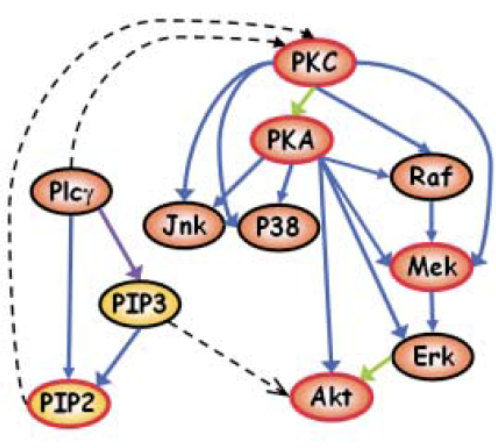
\includegraphics[scale=0.6]{sachs_network}
	\end{center}
	\caption{A DAG learned from phospho-protein/phospho-lipid expression data}
	\label{fig:prob6}
\end{figure}
This problem contains an analysis component and a programming component.

You are provided data that is drawn from the paper \cite{sachs2005causal} in the file \texttt{data.txt}. In this paper, the authors infer a protein-signaling network over the set of proteins/lipids that they measured. The resulting DAG is shown in Figure~\ref{fig:prob6}. One of the remarkable results of the paper was the exact reconstruction of the protein kinase cascade $\text{Raf} \diedgeright \text{Mek} \diedgeright \text{Erk}$, including the absence of direct regulation between Raf and Erk, corresponding to the absence of $\text{Raf} \diedgeright \text{Erk}$. Your goal here is to see if you can recreate the latter finding (absence of direct regulation)  from the data they have provided. Assume all colors of edges (including dashed ones) in Figure~\ref{fig:prob6} are present in the null DAG.

1) Pick (and justify) which of the following is a valid test statistic for the causal null (5 points)
\begin{align*}
H_0:\  \text{Raf} \diedgeright \text{Erk is absent}.
\end{align*}
a) $\odds(\text{Raf}, \text{Erk} \mid \text{Mek})$\\
b) $\odds(\text{Raf}, \text{Erk} \mid \text{Mek, PKA, PKC})$

\problemAnswer{
Only the latter is a valid test statistic. $\odds(\text{Raf}, \text{Erk} \mid \text{Mek})$ is not because conditioning on Mek opens a path from Raf to PKA to Erk, so the two variables being tested are not d-separated (a necessary condition for a test statistic to be valid). Observing PKA blocks this path, so  $\odds(\text{Raf}, \text{Erk} \mid \text{Mek, PKA, PKC})$ is valid.
}

2) If you take a look at the data, you will notice that it consists of mostly continuous valued variables. This makes computing the odds ratio fairly difficult, unless we assume simple parametric models like linear Gaussian models. However, we expect biological relations to be non-linear. We will instead use a non-parametric conditional independence test called the ``Fast Conditional Independence Test (FCIT)'' described by \cite{chalupka2018fast}. Read the introduction of the paper till the end of Section 1.1 and Section 2 till the end of Section 2.1 to get a sense of what the test does. Write 2-3 sentences to provide your understanding (this does not need to be rigorous, just demonstrate you tried reading about the method.) (5 points)

\problemAnswer{
The key principle underlying this test is that under the assumption that $X \ci Y \mid Z$, then prediction of $Y$ from both $X$ and $Z$ will offer no improvement in accuracy as compared to prediction of $Y$ from $Z$ alone. To test this, they use decision tree regression to produce a user-defined number of train/test splits, each of which produces a score for prediction accuracy of $Y$ given (a) $Z$, and (b) both $X$ and $Z$. Then, they test the null hypothesis that the scores from sets (a) and (b) are on average equal using a one-sided t-test (which would indicate that $X \ci Y \mid Z$).
}

3) Instead of computing the $\odds$, use an implementation of FCIT from the \texttt{fcit} package as a non-parametric test of conditional independence for the causal null based on your answer to 1). The skeleton for the output of your program is provided in \texttt{hw2.py}.  Using a significance level of $\alpha=0.05$, interpret the output of whichever test you decided was valid. Report the p-value and interpretation in your writeup. (10 points)

\problemAnswer{
At $p=0.24$, we {\bf fail to reject} the null hypothesis that $\textrm{Raf} \ci \textrm{Erk} \mid \textrm{Mek, PKA, PKC}$. This supports the conclusion drawn from the paper that there is no direct edge from Raf to Erk, but as we never ``accept" the null hypothesis, we should not conclusively say that this direct edge is not present. Further investigation, especially through direct perturbation, was a strong addition to the paper as they sought to explain the computational results they (and we!) found. Notably, at $p=0.01$ we $would$ reject the null hypothesis that $\textrm{Raf} \ci \textrm{Erk} \mid \textrm{Mek}$, a potentially misleading conclusion that could be drawn from an invalid test statistic, since Raf is not d-separated from Erk after conditioning on Mek alone.
}

Helpful notes:
\begin{itemize}
	\item The capitalization of the variable names in the data file may not exactly match the capitalization of the variables shown in Figure~\ref{fig:prob6}. But it should be fairly easy to tell which one is which.
	\item The GitHub page for FCIT provides helpful usage and installation tips: \url{https://github.com/kjchalup/fcit}.
	\item The inputs to FCIT have to be \texttt{numpy} matrices. So make sure all your inputs are at least $n\times 1$ \texttt{numpy} matrices (not 1-d arrays) where $n$ is the number of samples of data.
	\item Don't worry too much if the p-value from your implementation does not perfectly fit the story of the $\text{Raf} \diedgeright \text{Mek} \diedgeright \text{Erk}$ cascade -- that is the point of re-examining the actual data and determining the robustness of the conclusion (\cite{sachs2005causal} used linear models.) The FCIT test can be quite sensitive to random number initialization. If you implement the method correctly, and interpret the number appropriately according to the given significance level, you will receive full points. You may also run FCIT a few times over to see how sensitive your final conclusion is, but this is not necessary.
\end{itemize}
\bibliographystyle{apalike}
\bibliography{references}


\end{document}
